\chapter{Introduction}

\section{Background}
\label{section:background}

To date, many large modern software are written in C/C++ programming languages, from operating system kernels such as Linux and FreeBSD, to user space applications, including databases (e.g. MySQL, MongoDB), web browsers (e.g. Firefox, Chromium) and video game engines (e.g. Unreal Engine).

C/C++ allows programmers to directly manipulate memory, which helps in building high performance software programs, however, it also leaves door open for potential security vulnerabilities \cite{BurowNathan2017CIPS}. Attackers may make use of oversights in the program (such as omission of input validation, array bounds checking, etc.) to corrupt memory, and divert the control-flow of the program away from its original legitimate region to execute malicious code.

\begin{figure}[ht]
    \centering
    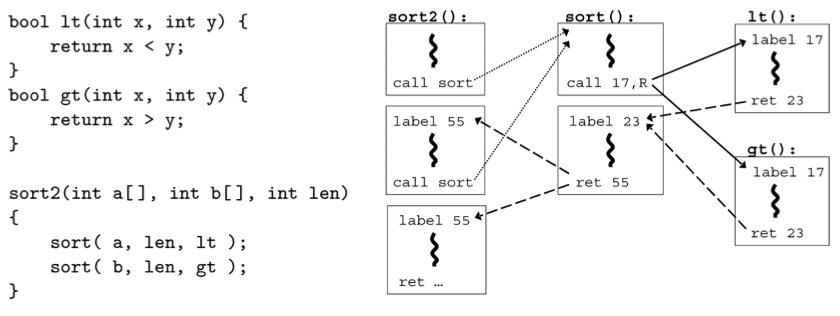
\includegraphics[keepaspectratio,width=0.65\paperwidth]{img/cfg.png}
    \caption{A piece of C code on the left, and its Control-Flow Graph \cite{cfi2005}.}
    \label{fig:cfg}
\end{figure}

In response, \ac{cfi} technique \cite{cfi2005} attempts to safeguard a program by restricting the control-flow of the program to its valid space \cite{nebelwelt}. The technique is composed of two phases, an ahead-of-time \textbf{analysis phase}, and a run-time \textbf{enforcement phase} \cite{BurowNathan2017CIPS}.

During analysis phase, static analysis is performed on source code or binary of the program to compute its \ac{cfg}, which basically represents the set of legitimate control-flow state transfers, such as function calls and returns.

Figure \ref{fig:cfg} illustrates an example of a control-flow graph. On the left, there is a piece of C code that contains three functions, \texttt{sort2()}, \texttt{lt()} and \texttt{gt()}. On the right is the control-flow graph of the source code. Nodes on the graph refer to functions in the program, and edges represent legitimate jumping from a location in a function to another location in another function.

More specifically, solid line arrows in the figure are called ``forward edge'', which represents a function call operation, where during the execution of a parent function, a child function is invoked and the program transfers to the child function. Dashed line arrows are called ``backward edge'', representing a return operation, where the child function returns to the parent caller function.

The control-flow graph in the figure illustrates that function \texttt{sort2()} may call function \texttt{sort()} at two locations in the middle of \texttt{sort2()}, and function \texttt{sort()} may call function \texttt{lt()} and function \texttt{gt()} in the middle of \texttt{sort()}. At the end of each children functions \texttt{sort()}, \texttt{lt()} and \texttt{gt()}, there is a backward edge returning to their parent call site.

After control-flow graph is constructed, during run-time enforcement phase, each control-flow state transfer is verified by checking whether there exists such an edge in CFG. If the transfer does not exist in the pre-computed CFG, then the control-flow integrity of the program must have been compromised, and actions can be taken, for example, terminate the program execution, send an alert to users and administrators, etc.

\section{Motivation}
\label{section:motivation}

Constructing control-flow graphs for programs like the one illustrated in Figure \ref{fig:cfg} is simple, because it only contains \ac{dfc}. Here ``direct function call'' refers to calling a function by its name, such as \texttt{memcpy(a, b, n);} and \texttt{fopen("file.txt", "r");}. In this case, it is sufficient to simply generate forward edges to \texttt{memcpy()} and \texttt{fopen()}, and backward edges returning to the paren caller function.

However, constructing control-flow graphs is much more complicated in the presence of \ac{ifc}. Indirect function calls are call operations to memory addresses instead of static function names. For instance, calling through a function pointer is an indirect function call.

Figure \ref{fig:fptr} illustrates an example of such a scenario. In the body of function \texttt{funcX()}, there is an indirect function call \texttt{p(2, 3);}, where \texttt{p} is not a function, but a function pointer. In this situation, static analysis is unable to immediately determine what is the target of the function call \texttt{p(2, 3);}, and hence unable to generate the control-flow graph for the program in Figure \ref{fig:fptr}.

\begin{figure}[h]
    \centering
    \begin{lstlisting}[language=c]
// Defines function pointer type
typedef int (*fptr_t)(int, int);

// Defines two functions of the type
int funcA(int a, int b) { return a + b; }
int funcB(int a, int b) { return a * b; }

// An indirect call happens here
int funcX(fptr_t p) { return p(2, 3); }

int main() { return funcX(&funcA); }
    \end{lstlisting}
    \caption{An example of function pointers and indirect function call}
    \label{fig:fptr}
\end{figure}

\newpage

Function pointers are extensively used in practical software development. For example, in Linux kernel, in order to support \texttt{open()} system call on different file-systems, the kernel may store function pointers to the underlying implementations of such functionality for \texttt{ext4}, \texttt{xfs}, \texttt{btrfs}, etc., and dynamically invoke the corresponding underlying function during run-time depending on the file-system used \cite{mlta}.

Function pointers are even essential in C++ language to realize run-time polymorphism. Objects of different subclass types can be passed as pointers or references in their common superclass type, but when calling a virtual method of the superclass type, the overriden method implementations of each respective subclass are actually called. This is achieved by each class object maintaining a virtual function table that stores function pointers to the actual method implementations of the concrete type of the object. During run-time, when calling a virtual method of the class object, the program queries its virtual function table for the memory address of the method implementation to be called, and calls the method through this function pointer.

In order for control-flow integrity to be practically useful in real-world applications, indirect function calls have to be handled properly. Control-flow integrity without support for indirect function calls is like a safety net with holes here and there, where direct function calls are verified and protected, but indirect function calls are totally exposed unprotected. Study shows that the constructed control-flow graph is often erroneously too small and barely useful, if function pointers are ignored \cite{cfg-extract}.

If call targets of indirect function calls are captured in control-flow graphs, then control-flow integrity enforcement can also cover indirect function calls, so that the effectiveness of control-flow protection is greatly improved. However, this is a hard problem, and in practice it is almost impossible to find call targets of indirect function calls in one hundred percent accuracy. Nonetheless, it is desirable to resolve targets of indirect function calls as precisely as possible, so the effectiveness of control-flow integrity enforcement is better than not covering indirect function calls at all, while not causing much performance overhead. Chapter \ref{chapter:previous-work} presents some of the existing approaches in doing so.

\section{Objective}
\label{section:objective}

This project aims to more accurately refine targets of indirect calls on function pointers, in the context of control-flow graph construction in C++ programs.

The scope of this project includes system and algorithm design, code implementation, results evaluation and comparison to other approaches.

In the end, this project will deliver a static analysis tool that performs function pointer targets analysis on C++ programs.

\section{Report Outline}
\label{section:outline}

The structure of this report in the following sections is organized as follows. Chapter \ref{chapter:previous-work} discusses some of the previous work in the field of analyzing the targets of indirect calls through function pointers in software programs, including simple type matching, and the state-of-the-art approach called multi-layer type analysis. Chapter \ref{chapter:methodology} introduces the methodology used in the project. Chapter \ref{chapter:status} presents current project status. Finally, chapter \ref{chapter:conclusion} concludes this project progress report in the end.